% Options for packages loaded elsewhere
\PassOptionsToPackage{unicode}{hyperref}
\PassOptionsToPackage{hyphens}{url}
\PassOptionsToPackage{dvipsnames,svgnames,x11names}{xcolor}
%
\documentclass[
  a4paper,
  DIV=11,
  numbers=noendperiod]{scrartcl}

\usepackage{amsmath,amssymb}
\usepackage{setspace}
\usepackage{iftex}
\ifPDFTeX
  \usepackage[T1]{fontenc}
  \usepackage[utf8]{inputenc}
  \usepackage{textcomp} % provide euro and other symbols
\else % if luatex or xetex
  \usepackage{unicode-math}
  \defaultfontfeatures{Scale=MatchLowercase}
  \defaultfontfeatures[\rmfamily]{Ligatures=TeX,Scale=1}
\fi
\usepackage{lmodern}
\ifPDFTeX\else  
    % xetex/luatex font selection
\fi
% Use upquote if available, for straight quotes in verbatim environments
\IfFileExists{upquote.sty}{\usepackage{upquote}}{}
\IfFileExists{microtype.sty}{% use microtype if available
  \usepackage[]{microtype}
  \UseMicrotypeSet[protrusion]{basicmath} % disable protrusion for tt fonts
}{}
\makeatletter
\@ifundefined{KOMAClassName}{% if non-KOMA class
  \IfFileExists{parskip.sty}{%
    \usepackage{parskip}
  }{% else
    \setlength{\parindent}{0pt}
    \setlength{\parskip}{6pt plus 2pt minus 1pt}}
}{% if KOMA class
  \KOMAoptions{parskip=half}}
\makeatother
\usepackage{xcolor}
\usepackage[headheight = 0 in,top = 1in,left = 0.8in,right =
0.8in,heightrounded]{geometry}
\setlength{\emergencystretch}{3em} % prevent overfull lines
\setcounter{secnumdepth}{-\maxdimen} % remove section numbering
% Make \paragraph and \subparagraph free-standing
\ifx\paragraph\undefined\else
  \let\oldparagraph\paragraph
  \renewcommand{\paragraph}[1]{\oldparagraph{#1}\mbox{}}
\fi
\ifx\subparagraph\undefined\else
  \let\oldsubparagraph\subparagraph
  \renewcommand{\subparagraph}[1]{\oldsubparagraph{#1}\mbox{}}
\fi

\usepackage{color}
\usepackage{fancyvrb}
\newcommand{\VerbBar}{|}
\newcommand{\VERB}{\Verb[commandchars=\\\{\}]}
\DefineVerbatimEnvironment{Highlighting}{Verbatim}{commandchars=\\\{\}}
% Add ',fontsize=\small' for more characters per line
\usepackage{framed}
\definecolor{shadecolor}{RGB}{241,243,245}
\newenvironment{Shaded}{\begin{snugshade}}{\end{snugshade}}
\newcommand{\AlertTok}[1]{\textcolor[rgb]{0.68,0.00,0.00}{#1}}
\newcommand{\AnnotationTok}[1]{\textcolor[rgb]{0.37,0.37,0.37}{#1}}
\newcommand{\AttributeTok}[1]{\textcolor[rgb]{0.40,0.45,0.13}{#1}}
\newcommand{\BaseNTok}[1]{\textcolor[rgb]{0.68,0.00,0.00}{#1}}
\newcommand{\BuiltInTok}[1]{\textcolor[rgb]{0.00,0.23,0.31}{#1}}
\newcommand{\CharTok}[1]{\textcolor[rgb]{0.13,0.47,0.30}{#1}}
\newcommand{\CommentTok}[1]{\textcolor[rgb]{0.37,0.37,0.37}{#1}}
\newcommand{\CommentVarTok}[1]{\textcolor[rgb]{0.37,0.37,0.37}{\textit{#1}}}
\newcommand{\ConstantTok}[1]{\textcolor[rgb]{0.56,0.35,0.01}{#1}}
\newcommand{\ControlFlowTok}[1]{\textcolor[rgb]{0.00,0.23,0.31}{#1}}
\newcommand{\DataTypeTok}[1]{\textcolor[rgb]{0.68,0.00,0.00}{#1}}
\newcommand{\DecValTok}[1]{\textcolor[rgb]{0.68,0.00,0.00}{#1}}
\newcommand{\DocumentationTok}[1]{\textcolor[rgb]{0.37,0.37,0.37}{\textit{#1}}}
\newcommand{\ErrorTok}[1]{\textcolor[rgb]{0.68,0.00,0.00}{#1}}
\newcommand{\ExtensionTok}[1]{\textcolor[rgb]{0.00,0.23,0.31}{#1}}
\newcommand{\FloatTok}[1]{\textcolor[rgb]{0.68,0.00,0.00}{#1}}
\newcommand{\FunctionTok}[1]{\textcolor[rgb]{0.28,0.35,0.67}{#1}}
\newcommand{\ImportTok}[1]{\textcolor[rgb]{0.00,0.46,0.62}{#1}}
\newcommand{\InformationTok}[1]{\textcolor[rgb]{0.37,0.37,0.37}{#1}}
\newcommand{\KeywordTok}[1]{\textcolor[rgb]{0.00,0.23,0.31}{#1}}
\newcommand{\NormalTok}[1]{\textcolor[rgb]{0.00,0.23,0.31}{#1}}
\newcommand{\OperatorTok}[1]{\textcolor[rgb]{0.37,0.37,0.37}{#1}}
\newcommand{\OtherTok}[1]{\textcolor[rgb]{0.00,0.23,0.31}{#1}}
\newcommand{\PreprocessorTok}[1]{\textcolor[rgb]{0.68,0.00,0.00}{#1}}
\newcommand{\RegionMarkerTok}[1]{\textcolor[rgb]{0.00,0.23,0.31}{#1}}
\newcommand{\SpecialCharTok}[1]{\textcolor[rgb]{0.37,0.37,0.37}{#1}}
\newcommand{\SpecialStringTok}[1]{\textcolor[rgb]{0.13,0.47,0.30}{#1}}
\newcommand{\StringTok}[1]{\textcolor[rgb]{0.13,0.47,0.30}{#1}}
\newcommand{\VariableTok}[1]{\textcolor[rgb]{0.07,0.07,0.07}{#1}}
\newcommand{\VerbatimStringTok}[1]{\textcolor[rgb]{0.13,0.47,0.30}{#1}}
\newcommand{\WarningTok}[1]{\textcolor[rgb]{0.37,0.37,0.37}{\textit{#1}}}

\providecommand{\tightlist}{%
  \setlength{\itemsep}{0pt}\setlength{\parskip}{0pt}}\usepackage{longtable,booktabs,array}
\usepackage{calc} % for calculating minipage widths
% Correct order of tables after \paragraph or \subparagraph
\usepackage{etoolbox}
\makeatletter
\patchcmd\longtable{\par}{\if@noskipsec\mbox{}\fi\par}{}{}
\makeatother
% Allow footnotes in longtable head/foot
\IfFileExists{footnotehyper.sty}{\usepackage{footnotehyper}}{\usepackage{footnote}}
\makesavenoteenv{longtable}
\usepackage{graphicx}
\makeatletter
\def\maxwidth{\ifdim\Gin@nat@width>\linewidth\linewidth\else\Gin@nat@width\fi}
\def\maxheight{\ifdim\Gin@nat@height>\textheight\textheight\else\Gin@nat@height\fi}
\makeatother
% Scale images if necessary, so that they will not overflow the page
% margins by default, and it is still possible to overwrite the defaults
% using explicit options in \includegraphics[width, height, ...]{}
\setkeys{Gin}{width=\maxwidth,height=\maxheight,keepaspectratio}
% Set default figure placement to htbp
\makeatletter
\def\fps@figure{htbp}
\makeatother

\KOMAoption{captions}{tableheading}
\makeatletter
\@ifpackageloaded{caption}{}{\usepackage{caption}}
\AtBeginDocument{%
\ifdefined\contentsname
  \renewcommand*\contentsname{Table of contents}
\else
  \newcommand\contentsname{Table of contents}
\fi
\ifdefined\listfigurename
  \renewcommand*\listfigurename{List of Figures}
\else
  \newcommand\listfigurename{List of Figures}
\fi
\ifdefined\listtablename
  \renewcommand*\listtablename{List of Tables}
\else
  \newcommand\listtablename{List of Tables}
\fi
\ifdefined\figurename
  \renewcommand*\figurename{Figure}
\else
  \newcommand\figurename{Figure}
\fi
\ifdefined\tablename
  \renewcommand*\tablename{Table}
\else
  \newcommand\tablename{Table}
\fi
}
\@ifpackageloaded{float}{}{\usepackage{float}}
\floatstyle{ruled}
\@ifundefined{c@chapter}{\newfloat{codelisting}{h}{lop}}{\newfloat{codelisting}{h}{lop}[chapter]}
\floatname{codelisting}{Listing}
\newcommand*\listoflistings{\listof{codelisting}{List of Listings}}
\makeatother
\makeatletter
\makeatother
\makeatletter
\@ifpackageloaded{caption}{}{\usepackage{caption}}
\@ifpackageloaded{subcaption}{}{\usepackage{subcaption}}
\makeatother
\ifLuaTeX
  \usepackage{selnolig}  % disable illegal ligatures
\fi
\usepackage{bookmark}

\IfFileExists{xurl.sty}{\usepackage{xurl}}{} % add URL line breaks if available
\urlstyle{same} % disable monospaced font for URLs
\hypersetup{
  pdftitle={IO2 PS2 Bresnahan and Reiss (1991)},
  pdfauthor={Carlos T. Estrada Arzamendi},
  colorlinks=true,
  linkcolor={blue},
  filecolor={Maroon},
  citecolor={Blue},
  urlcolor={Blue},
  pdfcreator={LaTeX via pandoc}}

\title{IO2 PS2 Bresnahan and Reiss (1991)}
\author{Carlos T. Estrada Arzamendi}
\date{March 25, 2024}

\begin{document}
\maketitle

\setstretch{1.25}
\section{Problem 1 :}\label{problem-1}

Reproduce the results for the tire dealers reported in Table 4 of the
paper. Note that Bresnahan and Reiss (1991) estimate the model imposing
the constraints \(\alpha_n \geq 0\) and \(\gamma_n \geq 0\). You should
impose the same constraints.

\begin{Shaded}
\begin{Highlighting}[numbers=left,,]
\CommentTok{\# Reading Data}
\NormalTok{data }\OtherTok{=} \FunctionTok{as.data.table}\NormalTok{(}\FunctionTok{read.csv}\NormalTok{(}\StringTok{"ps2.csv"}\NormalTok{))}
\end{Highlighting}
\end{Shaded}

\subsection{Reproducing Figure 2 to get to know the
data}\label{reproducing-figure-2-to-get-to-know-the-data}

\begin{Shaded}
\begin{Highlighting}[numbers=left,,]
\NormalTok{figure2 }\OtherTok{=} \FunctionTok{ggplot}\NormalTok{(data, }\FunctionTok{aes}\NormalTok{(}\AttributeTok{x =}\NormalTok{ TPOP)) }\SpecialCharTok{+} 
                \FunctionTok{geom\_histogram}\NormalTok{(}\AttributeTok{breaks =} \FunctionTok{seq}\NormalTok{(}\DecValTok{0}\NormalTok{,}\FloatTok{7.5}\NormalTok{, }\AttributeTok{by =} \FloatTok{0.5}\NormalTok{)) }\SpecialCharTok{+} 
                \FunctionTok{scale\_x\_continuous}\NormalTok{(}\AttributeTok{limits =} \FunctionTok{c}\NormalTok{(}\DecValTok{0}\NormalTok{, }\FloatTok{7.5}\NormalTok{), }\AttributeTok{oob =}\NormalTok{ scales}\SpecialCharTok{::}\NormalTok{oob\_squish) }\SpecialCharTok{+}
                \FunctionTok{xlab}\NormalTok{(}\StringTok{"Town Population (thousands)"}\NormalTok{) }\SpecialCharTok{+}
                \FunctionTok{ylab}\NormalTok{(}\StringTok{"Number of Towns"}\NormalTok{)}
\NormalTok{figure2}
\end{Highlighting}
\end{Shaded}

\begin{figure}[H]

{\centering 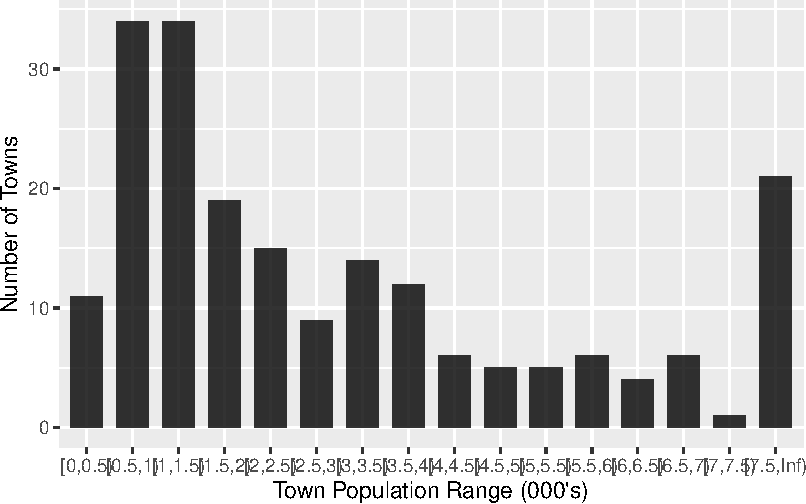
\includegraphics[width=0.6\textwidth,height=\textheight]{IO2_PS2_Estrada_files/figure-pdf/figure2-1.pdf}

}

\caption{Number of towns by town population}

\end{figure}%

\subsection{Reproducing Table 3 to get to know the
data}\label{reproducing-table-3-to-get-to-know-the-data}

\begin{Shaded}
\begin{Highlighting}[numbers=left,,]
\FunctionTok{datasummary\_skim}\NormalTok{(data, }\AttributeTok{out =} \StringTok{"markdown"}\NormalTok{, }\AttributeTok{histogram =}\NormalTok{ F, }\AttributeTok{title =} \StringTok{"Replication of Table 3"}\NormalTok{)}
\end{Highlighting}
\end{Shaded}

\begin{longtable}[]{@{}
  >{\raggedright\arraybackslash}p{(\columnwidth - 14\tabcolsep) * \real{0.0897}}
  >{\raggedleft\arraybackslash}p{(\columnwidth - 14\tabcolsep) * \real{0.1026}}
  >{\raggedleft\arraybackslash}p{(\columnwidth - 14\tabcolsep) * \real{0.1795}}
  >{\raggedleft\arraybackslash}p{(\columnwidth - 14\tabcolsep) * \real{0.1282}}
  >{\raggedleft\arraybackslash}p{(\columnwidth - 14\tabcolsep) * \real{0.1282}}
  >{\raggedleft\arraybackslash}p{(\columnwidth - 14\tabcolsep) * \real{0.1154}}
  >{\raggedleft\arraybackslash}p{(\columnwidth - 14\tabcolsep) * \real{0.1282}}
  >{\raggedleft\arraybackslash}p{(\columnwidth - 14\tabcolsep) * \real{0.1282}}@{}}
\caption{Replication of Table 3}\tabularnewline
\toprule\noalign{}
\begin{minipage}[b]{\linewidth}\raggedright
\end{minipage} & \begin{minipage}[b]{\linewidth}\raggedleft
Unique
\end{minipage} & \begin{minipage}[b]{\linewidth}\raggedleft
Missing Pct.
\end{minipage} & \begin{minipage}[b]{\linewidth}\raggedleft
Mean
\end{minipage} & \begin{minipage}[b]{\linewidth}\raggedleft
SD
\end{minipage} & \begin{minipage}[b]{\linewidth}\raggedleft
Min
\end{minipage} & \begin{minipage}[b]{\linewidth}\raggedleft
Median
\end{minipage} & \begin{minipage}[b]{\linewidth}\raggedleft
Max
\end{minipage} \\
\midrule\noalign{}
\endfirsthead
\toprule\noalign{}
\begin{minipage}[b]{\linewidth}\raggedright
\end{minipage} & \begin{minipage}[b]{\linewidth}\raggedleft
Unique
\end{minipage} & \begin{minipage}[b]{\linewidth}\raggedleft
Missing Pct.
\end{minipage} & \begin{minipage}[b]{\linewidth}\raggedleft
Mean
\end{minipage} & \begin{minipage}[b]{\linewidth}\raggedleft
SD
\end{minipage} & \begin{minipage}[b]{\linewidth}\raggedleft
Min
\end{minipage} & \begin{minipage}[b]{\linewidth}\raggedleft
Median
\end{minipage} & \begin{minipage}[b]{\linewidth}\raggedleft
Max
\end{minipage} \\
\midrule\noalign{}
\endhead
\bottomrule\noalign{}
\endlastfoot
ID & 202 & 0 & 328090.8 & 143299.0 & 40013.0 & 320014.0 & 560045.0 \\
TIRE & 14 & 0 & 2.6 & 2.6 & 0.0 & 2.0 & 13.0 \\
TPOP & 195 & 0 & 3.7 & 5.4 & 0.1 & 2.1 & 45.1 \\
NGRW & 58 & 0 & -0.1 & 0.1 & -1.3 & 0.0 & 0.0 \\
PGRW & 119 & 0 & 0.5 & 1.1 & 0.0 & 0.1 & 7.2 \\
OCTY & 160 & 0 & 0.3 & 0.7 & 0.0 & 0.2 & 8.4 \\
OPOP & 178 & 0 & 0.4 & 0.7 & 0.0 & 0.1 & 5.8 \\
LANDV & 166 & 0 & 0.3 & 0.2 & 0.1 & 0.2 & 1.6 \\
ELD & 198 & 0 & 0.1 & 0.0 & 0.0 & 0.1 & 0.3 \\
FFRAC & 174 & 0 & 0.7 & 0.4 & 0.0 & 0.8 & 1.3 \\
PINC & 191 & 0 & 5.9 & 1.1 & 3.2 & 5.9 & 10.5 \\
LNHDD & 62 & 0 & 8.6 & 0.5 & 6.8 & 8.7 & 9.2 \\
\end{longtable}

\subsection{Main Task: Table 4}\label{main-task-table-4}

\begin{Shaded}
\begin{Highlighting}[numbers=left,,]
\NormalTok{loglike }\OtherTok{=} \ControlFlowTok{function}\NormalTok{(par, x)\{}
\NormalTok{lambda }\OtherTok{=}\NormalTok{ par[}\DecValTok{1}\SpecialCharTok{:}\DecValTok{4}\NormalTok{]}
\NormalTok{beta }\OtherTok{=}\NormalTok{ par[}\DecValTok{5}\SpecialCharTok{:}\DecValTok{8}\NormalTok{]}
\NormalTok{alpha }\OtherTok{=}\NormalTok{ par[}\DecValTok{9}\SpecialCharTok{:}\DecValTok{13}\NormalTok{]}
\NormalTok{gamma }\OtherTok{=}\NormalTok{ par[}\DecValTok{14}\SpecialCharTok{:}\DecValTok{19}\NormalTok{]}

\NormalTok{s }\OtherTok{=}\NormalTok{ x}\SpecialCharTok{$}\NormalTok{TPOP }\SpecialCharTok{+}\NormalTok{ lambda[}\DecValTok{1}\NormalTok{]}\SpecialCharTok{*}\NormalTok{x}\SpecialCharTok{$}\NormalTok{NRGW }\SpecialCharTok{+}\NormalTok{ lambda[}\DecValTok{2}\NormalTok{]}\SpecialCharTok{*}\NormalTok{x}\SpecialCharTok{$}\NormalTok{PGRW }\SpecialCharTok{+}\NormalTok{ lambda[}\DecValTok{3}\NormalTok{]}\SpecialCharTok{*}\NormalTok{x}\SpecialCharTok{$}\NormalTok{OCTY }\SpecialCharTok{+}\NormalTok{ lambda[}\DecValTok{4}\NormalTok{]}\SpecialCharTok{*}\NormalTok{x}\SpecialCharTok{$}\NormalTok{OPOP}


\NormalTok{\}}
\end{Highlighting}
\end{Shaded}




\end{document}
